\subsubsection*{6.16}
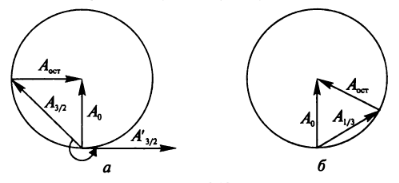
\includegraphics{parts/img/6_16.png}
На векторной диаграмме показаны амплитуды волн: в остутствие диска $A_0$, от полутора зон Френеля $A_{3/2}$, от зон вне диска $A_{ост.}$. Показатель преломления увеличивает фазу волны на $(2\pi / \lambda)(n - 1)h$. Максимум амплитуды в точке наблюдения будет, когда зона поворота $A_{3/2} = (5/4)\pi + 2\pi m $, где $m \in \mathbb{Z}^+$ (и $0$), откуда $h = (2m + 5/4)(\lambda/2)(n-1)$.